\begin{problem}{\#1 (20 points)}
    Consider the following CFG:\\
    $S \to AY | BZ | AA | BB$\\
    $Y \to SA$\\
    $Z \to SB$\\
    $A \to a$\\
    $B \to b$
    \begin{enumerate}[label=\alph*)]
        \item Find a derivation tree that does not have a self-embedded nonterminal.
        \item Find a derivation tree that contains a self-embedded nonterminal.
    \end{enumerate}
\end{problem}
\begin{solution}
    \begin{enumerate}[label=\alph*)]
        \item 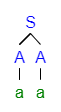
\includegraphics[width=0.12\linewidth]{figures/answer1a.png}
        \item 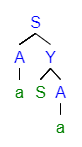
\includegraphics[width=0.15\linewidth]{figures/answer1b.png}
    \end{enumerate}
\end{solution}

\begin{problem}{\#2 (20 points)}
    Decide whether the following grammar generates any words using the algorithm of Theorem 43 (page 403) Chapter 18.
    \begin{enumerate}
        \item $S \to AB$\\
        $A \to BC | b$\\
        $C \to DA$\\
        $B \to CD$\\
        $D \to a$
        \item $S \to AB$\\
        $A \to BSB$\\
        $B \to AAS$\\
        $A \to CC$\\
        $B \to CC$\\
        $C \to SS$\\
        $A \to a|b$\\
        $C \to b|bb$
    \end{enumerate}
\end{problem}
\begin{solution}
    \begin{enumerate}
        \item First we replace the $D$ production everywhere with $a$.\\
        $S \to AB$\\
        $A \to BC | b$\\
        $C \to aA$\\
        $B \to Ca$\\
        Next we replace the $A$ production everywhere with $b$.\\
        $S \to bB$\\
        $C \to ab$\\
        $B \to Ca$\\
        Now we replace the $C$ production everywhere with $ab$\\
        $S \to bB$\\
        $B \to aba$\\
        Lastly we replace the $B$ production everywhere with $aba$.\\
        $S \to baba$\\
        There is a production of the form $S \to t$ so the language is not empty.
        \item First we replace the $C$ production with $b$\\
        $S \to AB$\\
        $A \to BSB$\\
        $B \to AAS$\\
        $A \to bb$\\
        $B \to bb$\\
        $A \to a|b$\\
        Next we replace all of the $B$ productions with $bb$.
        $S \to Abb$\\
        $A \to bbSbb$\\
        $A \to bb$\\
        $A \to a|b$\\
        Lastly we replace all of the $A$ productions with $a$.
        $S \to abb$\\
        There is a production of the form $S \to t$ so the language is not empty.
    \end{enumerate}
\end{solution}

\begin{problem}{\#3 (20 points)}
    Consider the following grammar for arithmetic expressions.
    \begin{align*}
        S &\to E\\
        E &\to T | E+T | E-T | -T\\
        T &\to F | T * F | T/F\\
        F &\to \left(E\right) | i
    \end{align*}
    Using top-down parsing, find a leftmost derivation in this grammar for the expression $i/i+i$. Show your work.
\end{problem}
\begin{solution}
\end{solution}

\begin{problem}{\#4 (20 points)}
    \begin{enumerate}[label=\alph*)]
        \item Consider the following Turing Machine (TM).
        \begin{figure}[H]
            \centering
            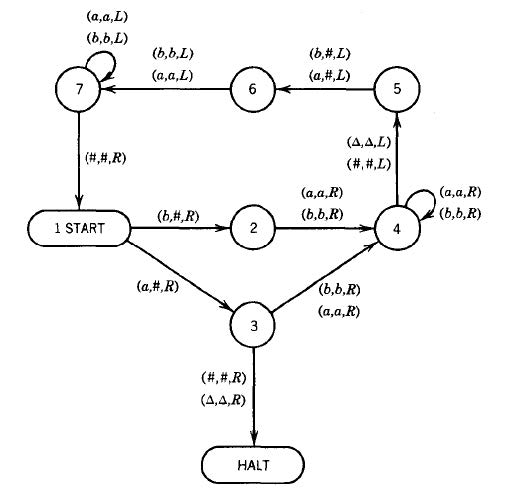
\includegraphics[width=0.8\linewidth]{figures/question4.jpg}
        \end{figure}
        Trace the execution chains of the following input strings on this machine.
        \begin{enumerate}[label=\arabic*)]
            \item baaba
            \item ababb
        \end{enumerate}
    \end{enumerate}
\end{problem}
\begin{solution}
    \begin{enumerate}[label=\alph*)]
        \item 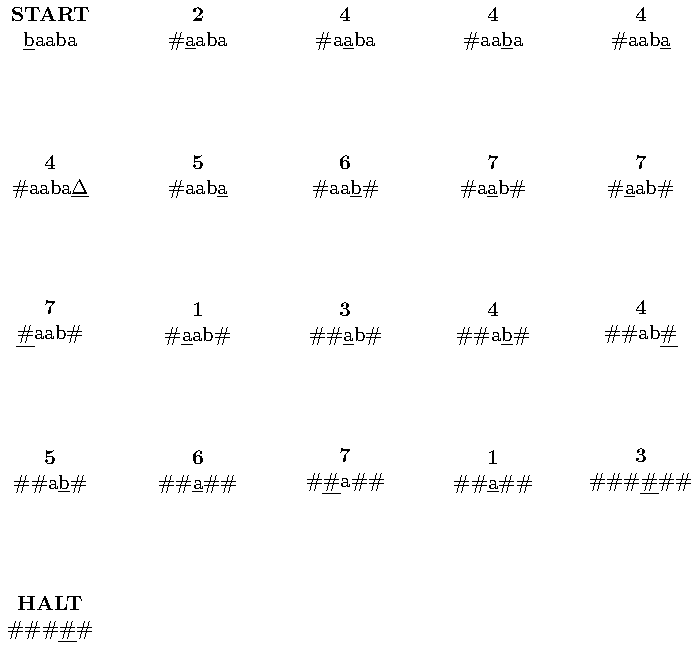
\includegraphics[]{figures/answer4a.pdf}
        \item 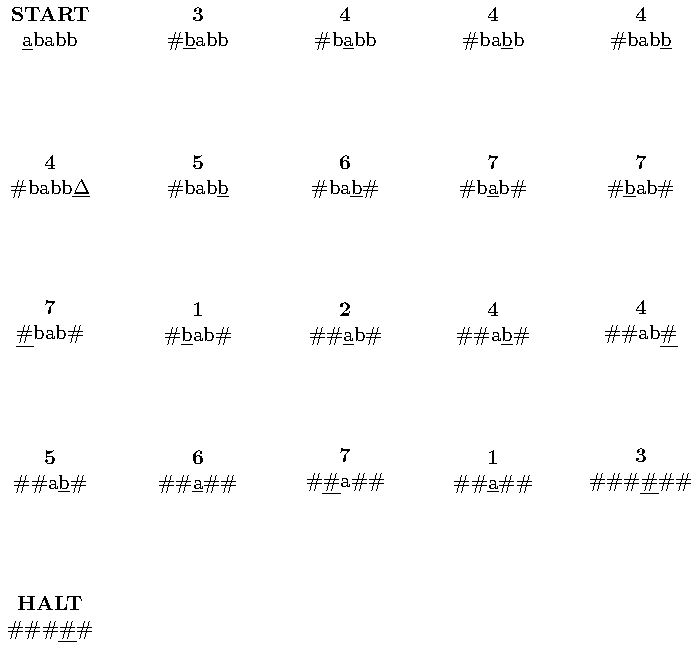
\includegraphics[]{figures/answer4b.pdf}
    \end{enumerate}
\end{solution}
